
\chapter{Simulating a biological neural network}

Up until now the inference of networks using NetRate has been used only on simulations. A random structure was generated and the spikes simulated using the Brian simulator. This is very useful because it allows the possibility of comparing the inferred network to a ground truth and evaluating the performance of the algorithm. However, the goal is to be able to implement NetRate on real biological networks whose topology could provide insight to scientists. The analysis of real biological neural networks is met with many difficulties that need to be dealt with.\\

The main problem regarding the inference of the connectivity of a biological neural network is the lack of a ground truth with which to compare the capabilities of the algorithm. Although never to a full extent, there are certain ways that can help deal with this issue. The first is to simulate a network that replicates the characteristics of the real one. Under the assumption that the simulated network has a similar behaviour (not necessarily same connections) to the biological one, the algorithm can be implemented and tested. Then, the accuracy obtained can be taken to be an approximation to the accuracy inferred real network. However, this is a very big assumption and in reality the simulated network is very different to the real one. However, the main reason for testing on a simulated network is to verify that any change in the stimulation model of the system or any new method of cascade generation is still valid. A deeper explanation of this topic will be given in section \ref{sec:number_of_spikes}.

Another way of measuring performance would be to separate the dataset into training and testing and running NetRate on the training set. With the resulting estimated weights, given that a set of neurons have fired at time \(t\), estimate the neuron with highest probability of spiking. The relevance of this analysis stems from the fact that if \(\alpha_{j,i}\) is high, then the probability of neuron \(i\) spiking given that neuron \(j\) has fired is also high. If the accuracy of prediction is sufficiently high, the network can be taken to be correctly inferred.\\

It is important to find a suitable dataset to analyse. It must either be made out of voltage readings from an array of sensors in a cluster of neurons or spike times and indices\footnote{Here, the index is the neuron number that generates a specific spike}. The second option is preferable because it would not require spike sorting. It would also be advantageous if the dataset contained some biological information as to the type of neurons present in the system, how they are connected (if there is any biological way of measuring it) or where they are located. This information would help in creating a reliable simulation of the system and having a way of estimating a ground truth. In the next section, the dataset that is going to be used will be discussed. 

\section{Mouse somatosensory cortex neuron dataset}

For this project, the dataset that will be studied is the CRNCNS mouse somatosensory cortex SSC-3 dataset \cite{ito2016spontaneous, ito2014large, litke2004does}. This is a recording of the spiking activity from a mouse's somatosensory cortex brain cells. These cells were grown in cultures for 2-4 weeks in vitro and 25 measurements of 1 hour were taken. The measurement method consisted of a 512 multi-electrode array	that sensed the voltage in the culture for each of the neurons. These recordings were then spike sorted using PCA. \\

The somatosensory cortex is a set of modules located in the neocortex in the brain. The neocortex is vital in giving humans many of its cognitive abilities such as language processing, logic, sensory perception and many others. The neocortex shares many of its characteristics and architecture across different species of animals which makes it a very interesting subject of study. The somatosensory cortex is special because it is responsible for the touch sensations and because its anatomy and physiology has been intensively investigated \cite{markram2015reconstruction}.\\

The dataset consists of 25 different 1 hour recordings with a varying number of neurons ranging from 98 to 594. The average number of spikes per neuron for all datasets is 2.1 Hz and the sampling frequency is 20 kHz. The dataset also contains additional information on the x-y coordinates of each of the neurons in the cultures. With all this information, it is of interest to analyse what the distribution of spikes is. Neurons with larger connections will spike more often than the rest. Figure \ref{fig:histogram_spikes} displays how the spikes are distributed in the network. It is clear that the number of spikes per neuron follows an exponential distribution. Most of the neurons have sparse connections and will fire less than 6000 times during the length of the recordings while a few neurons will fire many times due to their high connectivity. In the next section, a simulated network will be implemented that tries to mimic the observable characteristics of the real 98 neuron network.\\

\begin{figure}
	\centering
	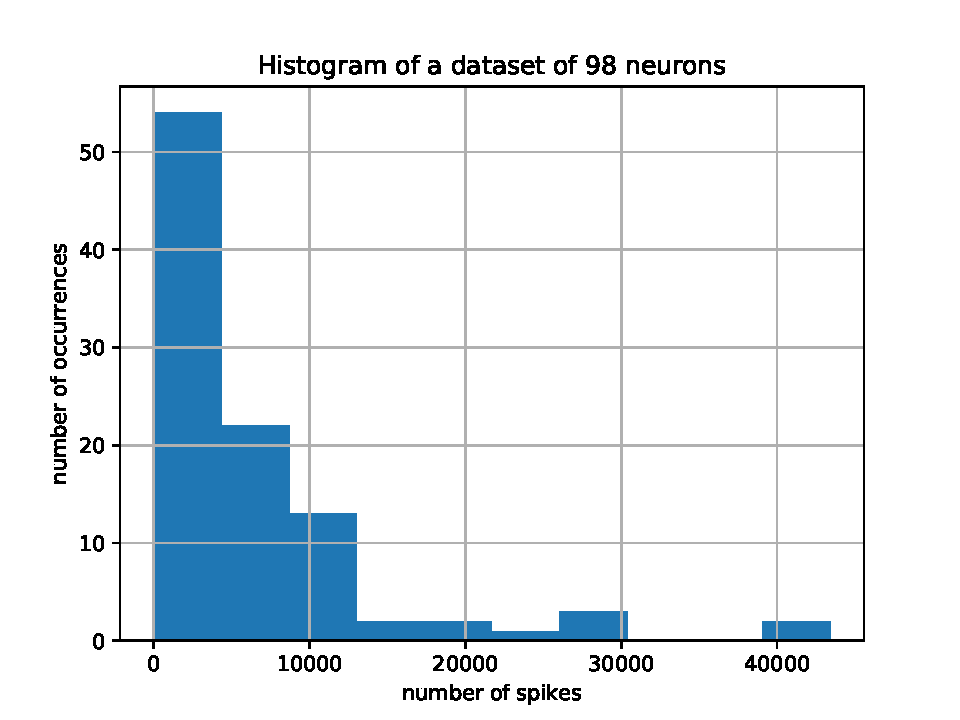
\includegraphics[width=0.8\textwidth]{histogram_number_spikes_dataset.pdf}
	\caption{Histogram of the number of spikes in a network of 98 neurons}
	\label{fig:histogram_spikes}
\end{figure}

\section{Input stimulus to the system}

Previous work \cite{alexandru2018estimating} simulated a network whose input was a DC voltage that stimulated each of the neurons one by one for a defined period of time (4 seconds). This proved to be very useful because it facilitated the analysis of each of the neurons regardless of their level of connectivity and because it provided a systematic way of generating cascades (more on this in section \ref{sec:simulating_cascade_generation}).
However, the neural system cultures from the dataset are not stimulated. Instead, they are left alone to interact between each other. The neurons then communicate independently of the outside environment and spike at a lower frequency as a result. \\

The input stimulus cannot be left unchanged because the behaviour of the network would be radically different to that of the real one. It cannot be null either because then no interactions between the neurons would occur. Some type of random input noise must be present in order to have spikes. Moreover, the new model should have biological significance since a real network is being replicated. An option is investigated that could potentially meet these requirements.\\

\subsection{System with random spikes}

The proposed model intends to mimic biological behaviour by assuming that neurons spike when they want to transmit some information that they have conveyed by themselves. In order to do so, a random neuron is selected from the network and stimulated with random noise for some length of time.\\

The noise that is input to the selected neuron is taken from the absolute value of a normal distribution of zero mean and standard deviation equal to \(\alpha ^{2}\). Since, a model of only excitatory neurons is being implemented, negative values from the distribution are not valid. 

The amount of time the selected neuron is stimulated for is also random. It is taken from a uniform distribution in the range 0 to 200 ms. There is no evidence to support the selection of this number since to this day, the behaviour of the neuron is not very well understood. However, it must be sufficiently large for the neuron to spike but to not too big so as to allow other neurons to be stimulated too. \\

The benefit of this model arises from its ability to insure that every neuron has roughly the same probability of originating a spike train, from its random behaviour in the system and from its major biological resemblance than the model used in \cite{alexandru2018estimating}.



\begin{figure}
	\centering
	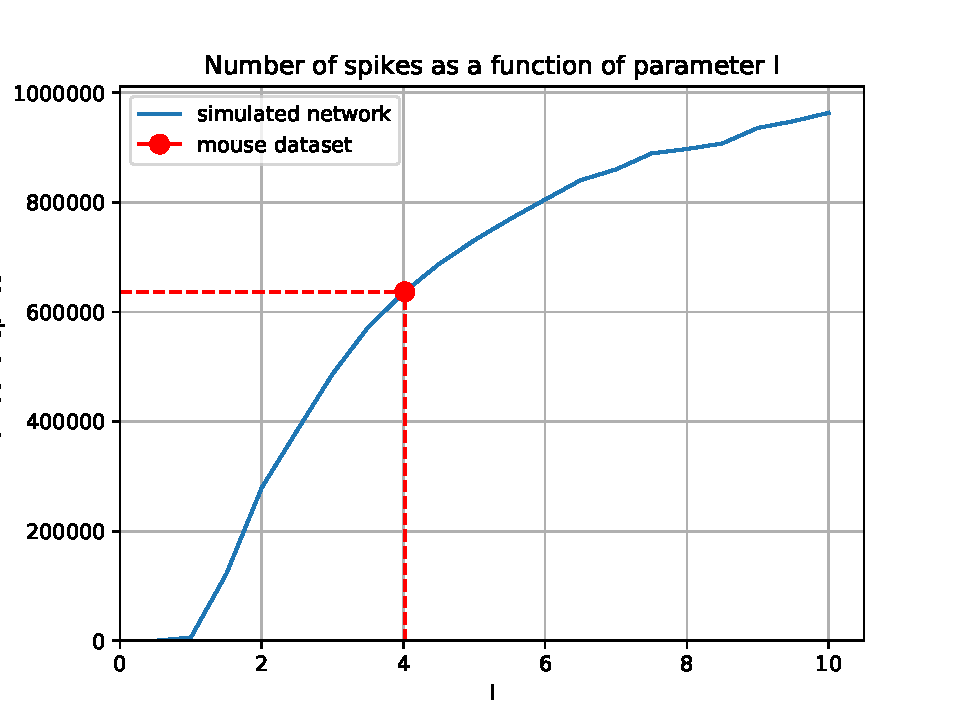
\includegraphics[width=0.8\textwidth]{I_var_plot.pdf}
	\caption{Number of spikes as a function of the parameter I for a 1 hour simulated network of 98 neurons and a random spike stimulus}
	\label{fig:I_var_plot}
\end{figure}

\section{Number of spikes}\label{sec:number_of_spikes}

At the beginning of this chapter the need for a simulated network that approximated the biological one was explained. Such a model can provide an approximation of performance of the algorithm. It is based on the assumption that the simulation is a faithful representation of the real nature of the network. Moreover, the differences between previous simulated networks and this new real network make it vital to verify that the algorithm would still work under these new conditions. 

\begin{table}[]
\centering
\begin{tabular}{|c|c|c|c|c|c|}
\hline
Type of network  & Neurons & Duration & Number of spikes & Mean    & Freq spikes/neuron \\ \hline
Real             & 98                & 3600 s           & 636878           & 6498.2  & 1.2 Hz               \\ \hline
Sim. DC stimulus & 98                & 392 s            & 4038313          & 41207.3 & 105.12 Hz            \\ \hline
\end{tabular}
\caption{Spike characteristics of different types of neural networks}
\label{tab:spike_characteristics}
\end{table}

As seen in table \ref{tab:spike_characteristics}, one of the most obvious changes with respect to previous simulations is the total number of spikes. This number is significantly smaller than before even though the observation time is larger. This is because the stimulation model forced the neurons to spike very frequently. In \cite{alexandru2018estimating} the total observation time was equal to the defined length of stimulation multiplied by the number of neurons. Since the stimulation period was found to be optimal for 4 seconds, then for a network of 98 neurons, this would result in a total of 392 seconds of recordings. 
On the other hand, the real dataset consists of recordings of one hour. Therefore, the model of the simulation must be such that the number of spikes is roughly the same for a 1 hour simulation length.


% Number of spikes
% 	I_var
% 	Frequency of spikes
% Shape of the histogram
% 	Changing the randomisation of the adjacency weights
% Types of neurons
% 	Excitatory and inhibitory
% 	What type of excitatory



\section{Cascade generation}\label{sec:simulating_cascade_generation}

Once the network model is defined what remains to clarify is how the cascades will be built. The method used in \cite{alexandru2018estimating} was simple and consistent. Since a DC stimulus was given to one neuron at a time, this neuron was selected to be the beginning of the cascade. This cascade would last for \(T\) length of time and only the first firing of each neuron would be taken into account. However, since the system no longer has a DC input, the cascade generation method must be changed. When selecting an appropriate method of cascade generation, certain factors are taken into account.
\begin{enumerate}
\item The higher the number of cascades that are generated, the more information will be conveyed and, in general, the better NetRate will be able to infer the connectivity of the network. 
\item The more separated the cascades are from each other in the time domain, the more independent they will be. Cascade independence is a critical characteristic of high quality cascade because it maximizes the likelihood of the spikes in the time horizon being caused by a previous spike in the same cascade.
\item A high sparsity insures that enough cascade information is obtained from all the neurons in the network. Otherwise, only neurons who spike often will be the ones generating cascades.
\end{enumerate}

\subsection{Method of maximum cascades}
\subsection{Method of maximum independence}
\subsection{Optimal cascade generation}
\section{Concluding remarks}

At the beginning of this chapter the need for a simulated network that approximated the biological one was explained. Such a model can provide an approximation of performance of the algorithm. It is based on the assumption that the simulation is a faithful representation of the real nature of the network. Moreover, the differences between previous simulated networks and this new real network make it vital to verify that the algorithm would still work under these new conditions. 
